\begin{figure}[H]
  \centering
  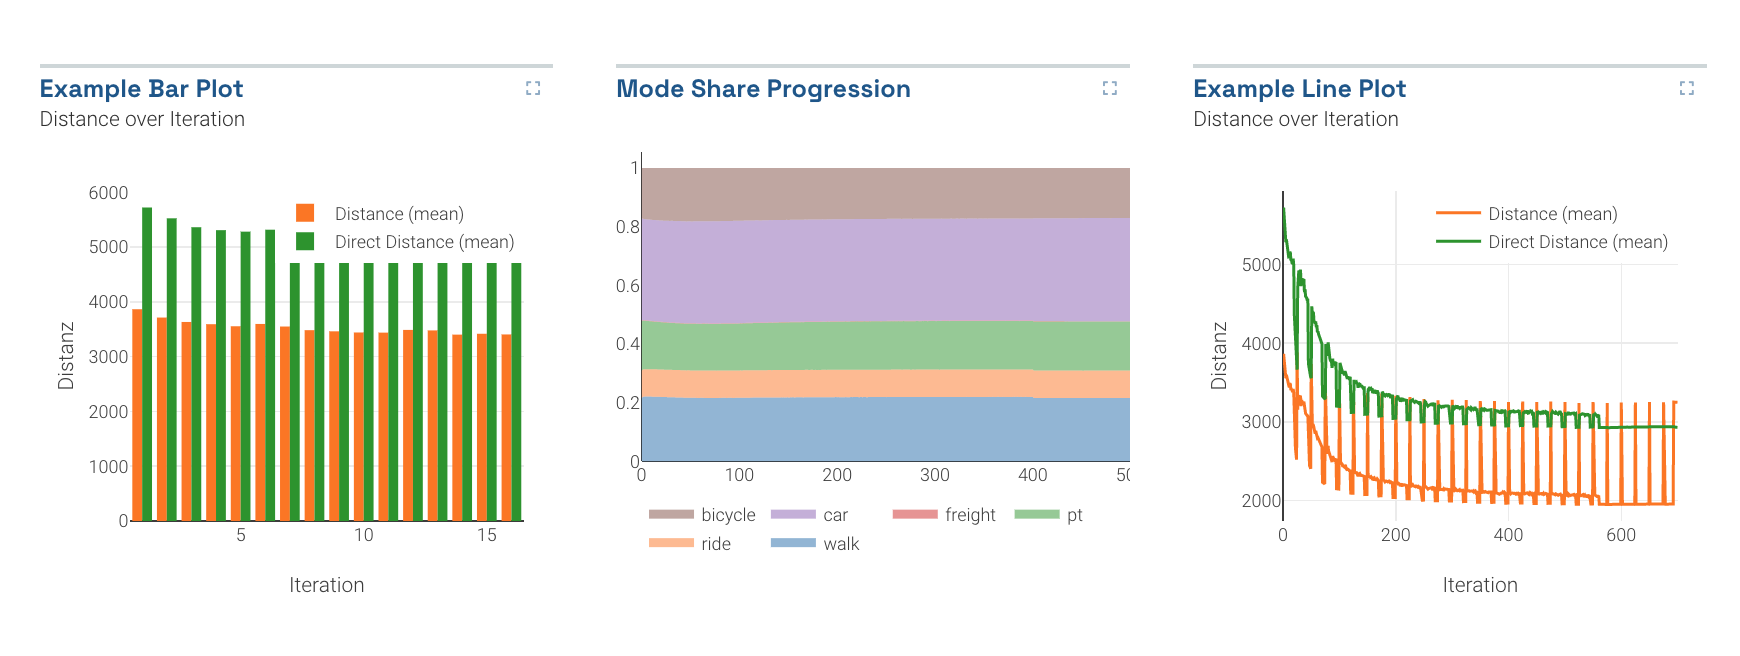
\includegraphics[width=0.8\textwidth]{assets/bar-line.png}
  \caption{Typical bar, area, and line charts}
\end{figure}

These simple charts comprise the core of many dashboards.

\hypertarget{usage}{%
\subsection{Usage}}

Bar, area, and line charts can only be included as panels in
\textbf{Dashboards}. See Dashboard documentation for general tips on
creating dashboard configurations.

\begin{itemize}
\tightlist
\item
  Each chart panel is defined inside a \textbf{row} in a
  \texttt{dashboard-*.yaml} file.
\item
  Choose from panel types \texttt{bar} \texttt{line} and \texttt{area}
  in the dashboard configuration.
\item
  Standard title, description, and width fields define the frame.
\end{itemize}

\begin{center}\rule{0.5\linewidth}{0.5pt}\end{center}

\hypertarget{sample-dashboard.yaml-config-snippet}{%
\subsubsection{Sample dashboard.yaml config
snippet}\label{sample-dashboard.yaml-config-snippet}}

\begin{lstlisting}
  layout:
  row1:
    - type: 'bar'
      title: 'Bar Plot'
      description: 'By iteration'
      width: 2
      dataset: '*drt_customer_stats.csv'
      x: 'iteration'
      xAxisName: 'Iteration'
      yAxisName: 'Distance'

    - type: 'area'
      title: 'Mode Share Progression'
      description: 'By iteration'
      width: 1
      dataset: '*modestats.txt'
      x: 'Iteration'

    - type: 'line'
      title: 'Mean Distances by Mode'
      description: 'per Iteration'
      width: 1
      dataset: '*drt_customer_stats.csv'
      x: 'iteration'
      xAxisName: 'Iteration'
      yAxisName: 'Distance'
      columns: [distance_m_mean, directDistance_m_mean]
      legendTitles: ['Distance (mean)', 'Direct Distance (mean)']

\end{lstlisting}

\hypertarget{bar-area-line-chart-properties}{%
\subsubsection{Bar, area, line chart properties}\label{bar-area-line-chart-properties}}

Each chart can have the following properties:

\noindent\textbf{dataset:} (Required) String. The filepath containing the data.
May include wildcards * and ?.

\noindent\textbf{x:} (Required) String. The column containing x-values.

\noindent\textbf{columns:} (Required) Array of strings. List the column names of
the columns which have the values to be graphed. Each element will be
its own line/color. Example:
\texttt{{[}\textquotesingle{}distance\textquotesingle{},\ \textquotesingle{}duration\textquotesingle{}{]}}

\noindent\textbf{useLastRow:} true/false. If set to true, only the last row of
the datafile will be used to build the pie chart. For example, this is
useful for MATSim outputs which list every iteration's output, and you
are only interested in the final iteration.

\noindent\textbf{stacked:} true/false for bar charts: whether to stack multiple
bars

\noindent\textbf{legendTitles:} Array of strings. Legend titles for each data
column. The column names will be used if this is omitted.

\noindent\textbf{xAxisName/yAxisName:} Labels for the axes.
